\chapter{Algoritmy}\label{ch:algoritmy}

%Popis společné části algoritmů (vstup, výstup).
%
%Stručný text o parametrech algoritmů.

Algoritmy tvoří plánující logiku křižovatky.
Jak bylo popsáno v~sekci \hyperref[sec:simulace]{simulace}, algoritmus hledá trasy pro~všechny agenty.
Každému úspěšně naplánovanému agentovi se přidělí nalezená trasa.

Všechny algoritmy podporují stejnou funkci \ref{alg:plan_agents},
kterou volá simulátor pro~nalezení tras agentů v~určitém kroku.
Vstup této funkce je krok simulace a množina agentů přijíždějících v~daném kroku.
Aby simulátor poznal, kterým agentům úspěšně přiřadil algoritmus trasu,
vrací funkce množinu úspěšně naplánovaných agentů.
Níže je zobrazen pseudokód výchozího chování funkce
\textrm{plan\_agents}\labeltext{\textrm{plan\_agents}}{alg:plan_agents}.

% @formatter:off
\begin{code}[xrightmargin=6em]
// vstup plánovaný krok step, množina agentů agents
// výstup množina naplánovaných agentů planned_agents
plan_agents(step, agents)
agents_mapped <- empty_set
for agent in agents
agents_mapped.add([agent, agent.entry, agent.exits])
return plan_agents(agents_mapped, step)
\end{code}
% @formatter:on

Všechny algoritmy podporují další pomocné funkce pro~zjednodušení a propojení algoritmů.
První pomocná funkce se~nazývá \ref{alg:plan_agent},
která má za~úkol naplánovat pouze jednoho agenta.
Tuto funkci využiji při~použití \ref{str:rs} strategie
(této strategii odpovídá výchozí implementace funkce \ref{alg:plan_agents}).
Funkce \textrm{plan\_agent}\labeltext{\textrm{plan\_agent}}{alg:plan_agent} dostává na~vstup krok, ve~kterém má~být agent naplánován.
Další parametry jsou agent, který má~být naplánován, vrchol,
ze~kterého agent vyjíždí a množina vrcholů, na~kterých může agent skončit.
Implementace funkce už~není jednotná a závisí na~každém algoritmu.
Funkce vrací agenta pokud byl úspěšně naplánován, jinak $NULL$.

% @formatter:off
\begin{code}[xrightmargin=14em]
// vstup plánovaný krok step, agent agent,
// vjezd entry a výjezdy exits
// výstup agent nebo NULL
plan_agent(step, agent, entry, exits)
// implementace algoritmu
if plánování úspěšné
agent.path <- planned_path
return agent
else
return NULL
\end{code}
% @formatter:on

Další pomocná funkce je rozšíření funkce \ref{alg:plan_agents}, která má na~vstupu krok plánování.
Další vstup je množina trojic, kde~první prvek trojice je agent, který má~být naplánován.
Další prvek je vrchol ze~kterého agent vyjíždí a
poslední prvek je množina cílových vrcholů, což jsou možné vrcholy, na~kterých má agent skončit.
Funkce opět vrací množinu naplánovaných agentů.
Pseudokód výchozího chování je následovný.
% @formatter:off
\begin{code}[xrightmargin=6em]
// vstup plánovaný krok step, množina trojic agentů,
// vjezdů a výjezdů agents_entries_exits
// výstup množina naplánovaných agentů planned_agents
plan_agents(step, agents_entries_exits)
planned_agents <- empty_set
for agent_entry_exits in agents_entries_exits
agent = agent_entry_exits[0]
entry = agent_entry_exits[1]
exists = agent_entry_exits[2]
planned_agent <- plan_agent(step, agent, entry, exists)
if planned_agent is not NULL
planned_agents.add(planned_agent)
return planned_agents
\end{code}
% @formatter:on

Implementované algoritmy mají různé nastavitelné parametry, které ovlivňují nalezené trasy, optimalitu či~dobu běhu.
Každý algoritmus má speciální parametry pro~něj vhodné.
Tyto~parametry proto budou popsány zvlášť a zároveň zvlášť testovány.

\section{Kontrola kolize}\label{sec:kolize}

%Rozbor případů, kdy může nastat mezi agenty kolize (základ v MAPF).
%Rozšíření problému na agenty s nenulovou velikostí.
%Popis pomocných datových struktur.

Při~hledání cest musí algoritmus brát v~potaz již naplánované agenty.
Pro tyto účely jsem si vytvořil následující pomocnou datovou strukturu, do které ukládám potřebné informace.

\paragraph{Tabulka obsazených pozic}\label{par:obsazene_pozice} si pamatuje pro~každý krok množinu dvojic vrcholu a agenta.
Díky této struktuře můžu jednoduše a rychle zjistit,
zda se v daný krok vyskytuje již naplánovaný agent na určeném vrcholu, a popřípadě o kterého agent se jedná.
Po~naplánování agenta je postupně přidána dvojice do~každého kroku, kdy se agent vyskytuje na~křižovatce.

Kontrola kolize probíhá třemi fázemi, kontroluje se~\nameref{subsec:bezpecnost_vrcholu},
\nameref{subsec:cesta_do_vrcholu} a \nameref{subsec:cesta_z_vrcholu}.

\paragraph{Safe distance}\label{par:safe_distance} (značený $d$) určuje minimální povolenou vzdálenost mezi dvěma agenty.
\nameref{par:safe_distance} je společný parametr všech kontrol a lze nastavit před~spuštěním simulace.
Nenulová hodnota \nameref{par:safe_distance} má šanci snížit kolize,
pokud jsou zavedené nepřesnosti parametrem \nameref{par:odchylka}.

Jelikož se můžou agenti v libovolný okamžik jakkoliv natočit, pracuji ve~výpočtech se zjednodušeným modelem agentů.
Namísto počítání složitého aktuálního natočení agenta a následné převedení na obdélník je agent nahrazen pomyslným kruhem.

\paragraph{Poloměr agenta}\label{par:polomer_agenta} určuje poloměr kruhu zjednodušeného modelu
a spočítá se z~agentovo délky~$l$ a šířky~$w$ jako $\frac{\sqrt {l^2 + w^2}}{2}$.
Kontroly poté zjišťují, jestli jsou kruhy tvořené pozicí agenta a jeho poloměrem disjunktní.
Jinými slovy agenti jsou kontrolami vyhodnoceni v~kolizních trasách
pokud se během cesty středy agentů přiblíží na~vzdálenost menší nebo rovnu součtu jejich poloměrů a \emph{safe distance}.
Toto zjednodušení nemůže způsobit kolizi, jelikož je celý agent umístěn uvnitř \hyperref[par:polomer_agenta]{poloměru agenta}.
Zároveň počítání s kruhem značně zrychluje samotný výpočet.

\subsection{Bezpečnost vrcholu}\label{subsec:bezpecnost_vrcholu}

%Popis postupu kontroly, pseudokód, náčrtek.

\hyperref[subsec:bezpecnost_vrcholu]{Kontrola bezpečnosti vrcholu} zjišťuje,
zda~je bezpečný výskyt agenta v~určitém kroku na~určeném vrcholu.
Kontrola je rozšíření první \ref{str:mapf} podmínky
\uv{žádní dva agenti se nesmí nacházet na stejném vrcholu v jednom kroku} \eqref{eq:mapf_kolize_vrchol}.

Tato kontrola pracuje s~vrcholem~$v$, krokem~$s$ a poloměrem agenta~$r$, pro kterého je kontrola určená.
Dále algoritmus zná maximální povolenou velikost agenta.
Z~této hodnoty je předpočítán maximální poloměr agenta~$m$.

Kontrola začne procházet všechny vrcholy grafu od~nejbližšího $v$ podle eukleidovské vzdálenosti.
Pro~každý vrchol~$u$, který je blíže než~$r + d + m$, se nejprve zjistí,
jestli je na~vrcholu~$u$ v~kroku~$s$ nějaký agent.
Pokud není, pokračuje kontrola dalším vrcholem.
Jinak se spočítá poloměr agenta~$r'$ nacházejícího se v~kroku~$s$ na~vrcholu~$u$.
Pokud je eukleidovská vzdálenost vrcholů $u$ a $v$ menší nebo rovna~$r + r' + d$, kontrola selže.
V~opačném případě přejde kontrola na~další vrchol.

Na obrázku (Obrázek~\ref{fig:kolize_na_vrcholu}) je ukázka situací, ve kterých tato kontrola selže.
Vlevo dochází ke kolizi, jelikož jsou dva agenti na stejném vrcholu.
Vpravo nastává situace, kdy jsou dva agenti příliš blízko.
Situace je kontrolou vyhodnocena jako kolizní i když se agenti nepřekrývají.

\begin{figure}[h]
  \centering
  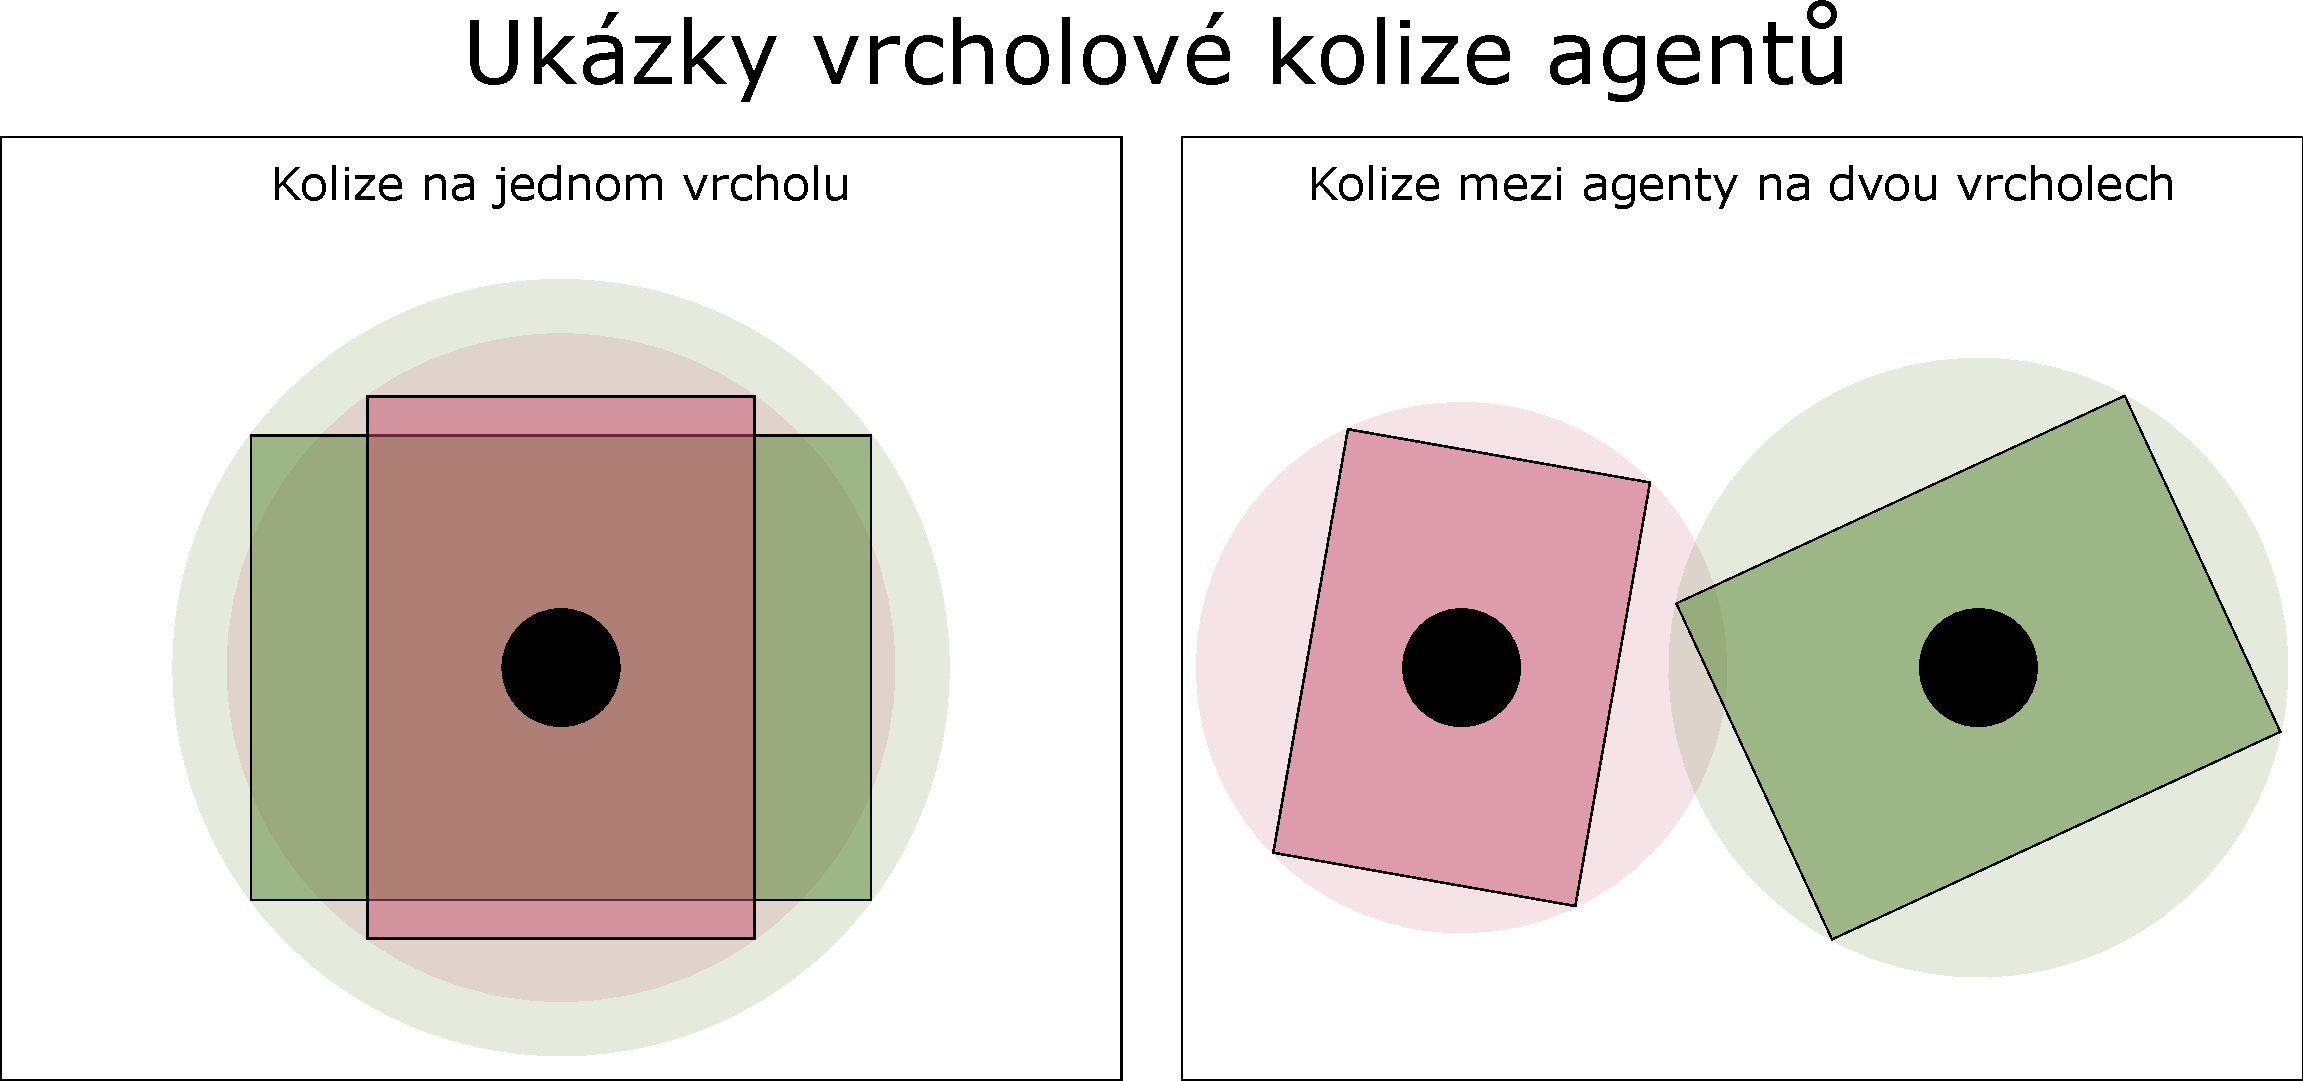
\includegraphics[width=\textwidth]{../img/kolize_vrchol}
  \caption{
    Ukázka kolizních situací, které jsou detekovány \hyperref[subsec:bezpecnost_vrcholu]{kontrolou bezpečnosti vrcholu}.
    Na obrázcích jsou černě zobrazeny vrcholy.
    Obdélníky reprezentují agenty a kruhy tvoří bezpečnou zónu příslušných agentů.
  }
  \label{fig:kolize_na_vrcholu}
\end{figure}

Níže je popsaný algoritmus na~kontrolu bezpečnosti vrcholu.
% @formatter:off
\begin{code}
// konstanty tabulka obsazených pozic t, minimální vzdálenost agentů d,
// maximální poloměr agenta m

// vstup krok s, vrchol v, poloměr agenta r
// výstup true pokud může agent být na v, jinak false
safe_vertex(s, v, r)
  for u in sorted(V, x -> dist(x, v))
    if dist(u, v) > r + m + d return true
    else
      n <- t[s][v]
      r' <- diameter(n)
      if dist(u, v) <= r + r' + d return false
  return true
\end{code}
% @formatter:on

\subsection{Cesta do~vrcholu}\label{subsec:cesta_do_vrcholu}

%Popis postupu kontroly, pseudokód, náčrtek.

\hyperref[subsec:cesta_do_vrcholu]{Kontrola cesty do vrcholu} zjišťuje,
zda~může plánovaný agent bezpečně přejet do~určeného vrcholu v~určitém kroku,
aniž by došlo ke kolizi s nějakým agentem opouštějícím daný vrchol.
Kontrola zahrnuje druhou \ref{str:mapf} podmínku
\uv{žádní dva agenti se nesmí projíždět stejnou hranou v jednom kroku} \eqref{eq:mapf_kolize_hrana}.
Avšak jelikož mají agenti nenulovou velikost, je nutné kontrolovat i případy, kdy agenti neprojíždí stejnou hranou.
Tyto situace jsou častější čím menší úhel je mezi sousedy vrcholu.
Například pro~čtvercový typ, kde je úhel mezi sousedy $90^\circ$, nastává tato kolize pouze pro velké agenty.
U~oktagonálního typu křižovatky dochází ke~kolizi mnohem častěji, protože úhel mezi sousedy činí $45^\circ$.
Ukázka kolizního stavu je zobrazena na obrázku (Obrázek~\ref{fig:kolize_cesta_do}).

\begin{figure}[h]
  \centering
  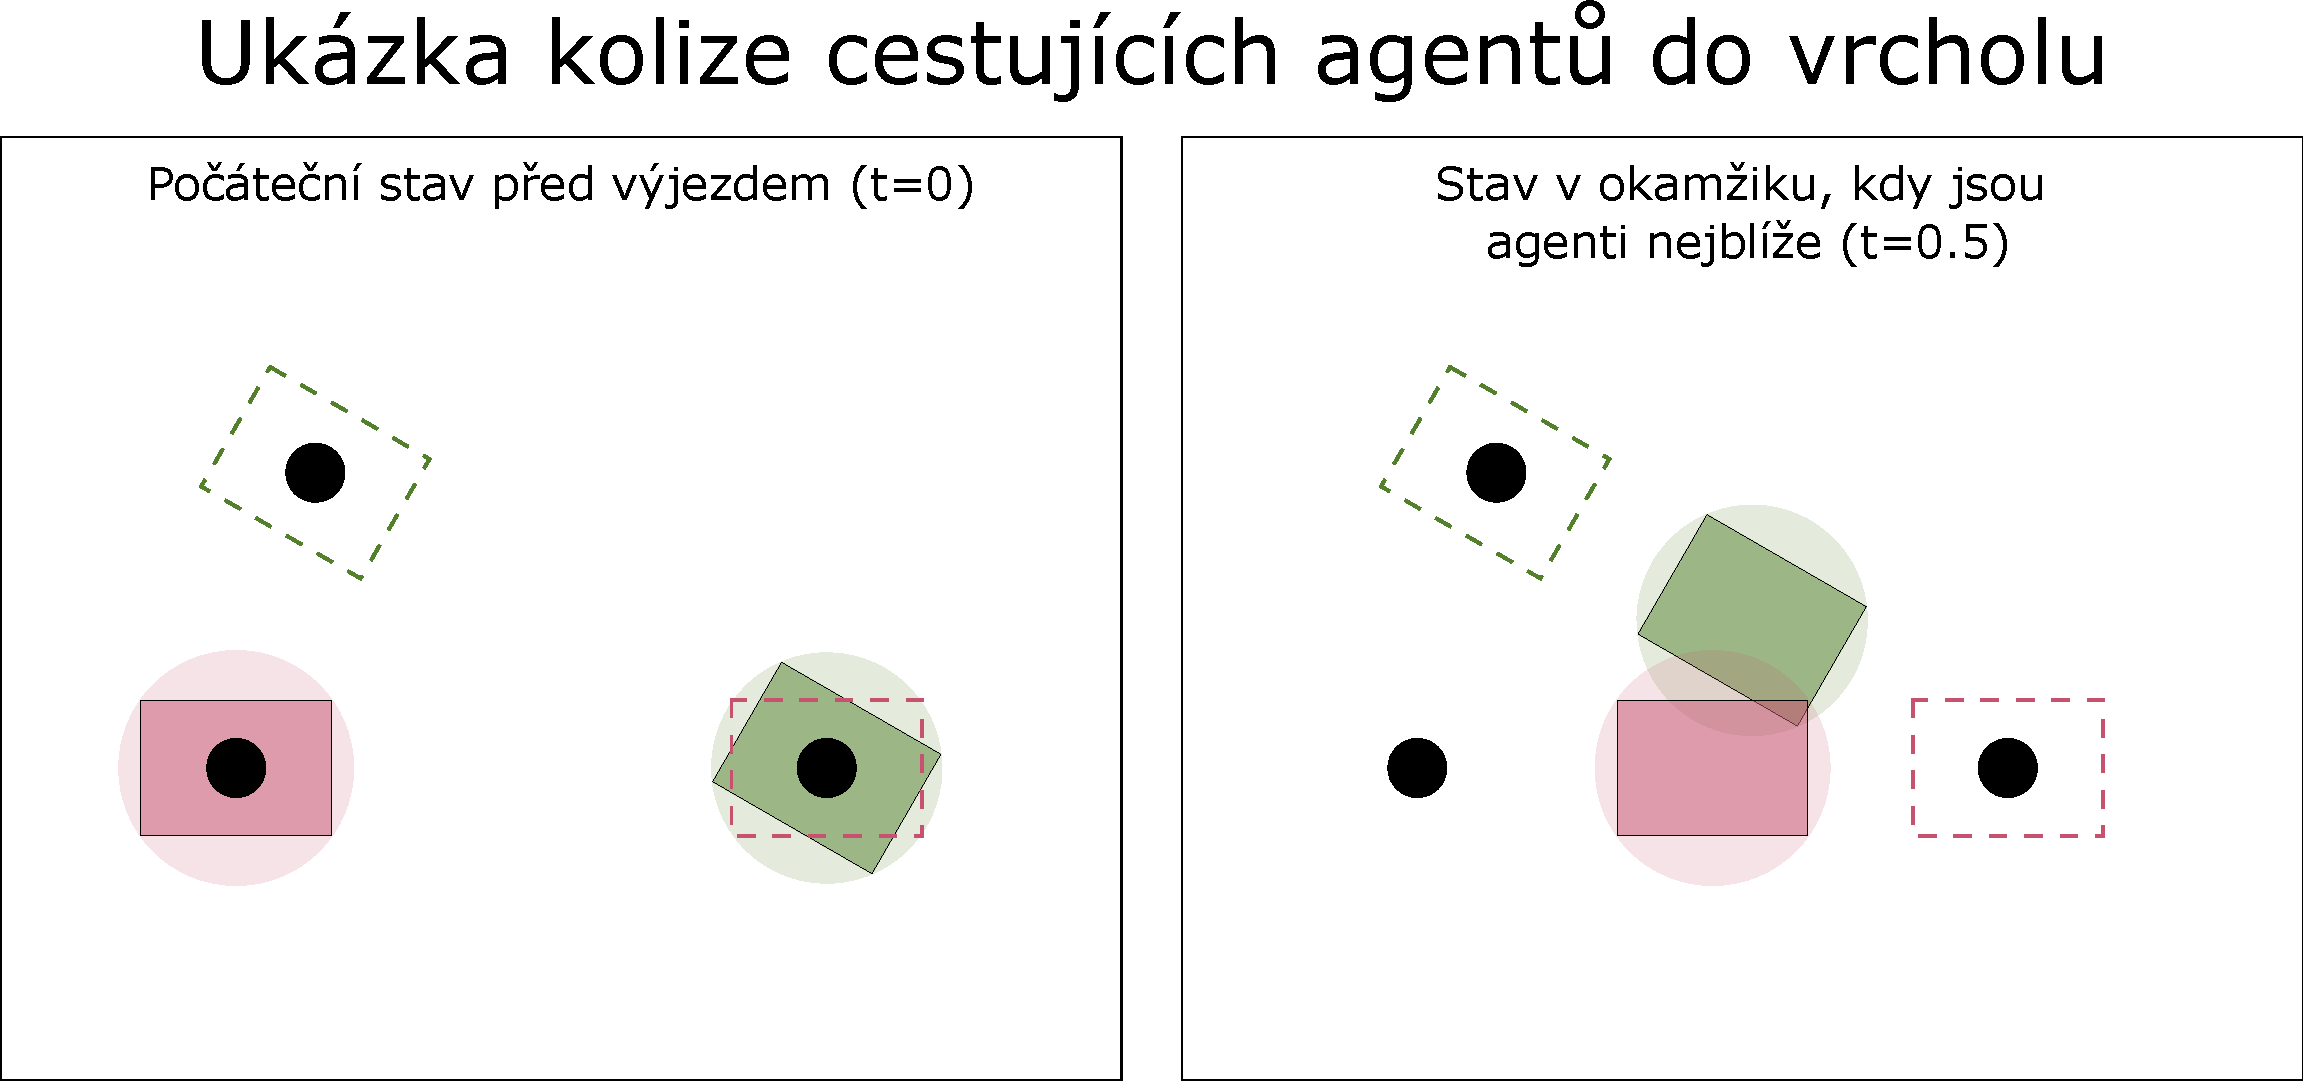
\includegraphics[width=\textwidth]{../img/kolize_cesta_do}
  \caption{
    Ukázka kolizní situace, která je detekována \hyperref[subsec:cesta_do_vrcholu]{kontrolou cesty do vrcholu}.
    Na obrázcích jsou černě zobrazeny vrcholy.
    Obdélníky reprezentují agenty a kruhy tvoří bezpečnou zónu příslušných agentů.
    Čárkované prázdné obdélníky značí cílové stavy agentů po jednom kroku.
  }
  \label{fig:kolize_cesta_do}
\end{figure}


Tato kontrola probíhá, pokud agent~$a$ opouští vrchol~$u$ v kroku~$s$ a přijíždí do~vrcholu~$v$ v následujícím kroku~$s + 1$.
Algoritmus nejprve zjistí, zda existuje naplánovaný agent~$b$, který je v~kroku~$s$ na~$v$.
Pokud žádný takový agent neexistuje, kontrola uspěje.
Jinak se zjistí vrchol~$w$, na~kterém se nachází agent~$b$ v~následujícím kroku $s + 1$.
Pokud nastane speciální případ $u=w$, odpovídá stav zmiňované \ref{str:mapf} podmínce \eqref{eq:mapf_kolize_hrana}.

Pokud se agenti srazí, musí být v kolizní poloze i v čase, kdy jsou sobě nejblíže.
Naopak pokud jsou dostatečně daleko i když jsou si nejblíže, při cestě nemůže dojít ke kolizi.
Jelikož kontrola zná pozice vrcholů $u$, $v$ a $w$, je schopna si dopočítat čas, ve~kterém se agenti nejvíce přiblíží.

Označím polohu agenta~$a$ jako $[x_a, y_a]$ a polohu agenta~$b$ jako $[x_b, y_b]$.
Stejným způsobem si označím pozice vrcholů $u$, $v$ a $w$ jako $[x_u, y_u]$, $[x_v, y_v]$ resp. $[x_w, y_w]$.
Dále si označím čas mezi kroky~$s$ a $s + 1$ jako~$t\in[0, 1]$.
Pro~$t = 0$ je poloha agenta~$a$ shodná s~pozicí vrcholu~$u$ a poloha agenta~$b$ shodná s~pozicí vrcholu~$v$.
Analogicky v~čase $t = 1$ se nachází agent~$a$ na~vrcholu~$v$ a agent~$b$ na~vrcholu~$w$.

Jelikož se agenti pohybují po~úsečce mezi vrcholy,
pro~$t\in[0, 1]$ se agent nachází na~$x_a = tx_u + (1 - t)x_v$, $y_a = ty_u + (1 - t)y_v$.
Poloha agenta~$b$ je analogicky $x_b = tx_v + (1 - t)x_w$ a $y_b = ty_v + (1 - t)y_w$.
Vzdálenost agentů v~závislosti na~čase~$t$ je $\sqrt{(x_a - x_b)^2 + (y_a - y_b)^2}$.
Dále upravím vzorec pod~odmocninou.
\begin{align*}
  ((x_a - x_b)^2 &+ (y_a - y_b)^2) = \\
  ((tx_u + (1 - t)x_v - tx_v - (1 - t)x_w)^2 &+ (ty_u + (1 - t)y_v - ty_v - (1 - t)y_w)^2) = \\
  ((tx_u + x_v - tx_v - tx_v - x_w + tx_w)^2 &+ (ty_u + y_v - ty_v - ty_v - y_w + ty_w)^2) = \\
  ((t(x_u - x_v - x_v + x_w) + x_v - x_w)^2 &+ (t(y_u - y_v - y_v + y_w) + y_v - y_w)^2) = \\
  (t(x_u - x_v - x_v + x_w) + x_v - x_w)^2 &+ (t(y_u - y_v - y_v + y_w) + y_v - y_w)^2 = \\
  (t(x_u - 2x_v + x_w) + x_v - x_w)^2 &+ (t(y_u - 2y_v + y_w) + y_v - y_w)^2 \\
\end{align*}

Pro~zjednodušení si označím
\begin{align*}
  x_0 &= x_u - 2x_v + x_w &\qquad
  x_1 &= x_w - x_v \\
  y_0 &= y_u - 2y_v + y_w &\qquad
  y_1 &= y_w - y_v
\end{align*}

Dosazením do~předchozího vzorce dostávám
\begin{align*}
  ((x_a - x_b)^2 &+ (y_a - y_b)^2) = \\
  (t(x_u - 2x_v + x_w) + x_v - x_w)^2 &+ (t(y_u - 2y_v + y_w) + y_v - y_w)^2 = \\
  (tx_0 - x_1)^2 &+ (ty_0 - y_1)^2
\end{align*}

Pro~nalezení nejmenší vzdálenosti zjistím čas~$t$, ve~kterém se agenti nacházejí nejblíže.
K~tomu spočítám derivaci vzdálenosti a zjistím, kdy je rovna nule.
Nejprve využiji faktu, že $\min\left(\sqrt{x}\right) = \min(x) \Rightarrow \frac{d}{dx} \sqrt {x} = 0 \leftrightarrow \frac{d}{dx} x=0$.
Následně
\begin{align}
  \frac{d}{dt} \sqrt{(x_a - x_b)^2 + (y_a - y_b)^2} &= 0 \nonumber \\
  \frac{d}{dt} ((x_a - x_b)^2 + (y_a - y_b)^2) &= 0 \nonumber \\
  \frac{d}{dt} ((tx_0 - x_1)^2 + (ty_0 - y_1)^2) &= 0 \nonumber \\
  \frac{d}{dt} (tx_0 - x_1)^2 + \frac{d}{dt} (ty_0 - y_1)^2 &= 0 \nonumber \\
  2(tx_0 - x_1)x_0 + 2(ty_0 - y_1)y_0 &= 0 \nonumber \\
  tx_0^2 - x_0 x_1 + ty_0 - y_0 y_1 &= 0 \nonumber \\
  t(x_0^2 + y_0^2) &= x_0 x_1 + y_0 + y_1 \label{eq:kol_d_dt}
\end{align}

Rozeberu dva případy podle podmínky
\begin{gather}
  x_0^2 + y_0^2 = 0\label{kol:nulova_podminka}
\end{gather}

Pokud je splněna podmínka~\ref{kol:nulova_podminka}, platí $x_0^2 = 0$ a $y_0^2 = 0$.
Odtud
\begin{align*}
  x_u - 2 x_v + x_w &= 0 \\
  x_u + x_w &= 2 x_v \\
  \frac{x_u + x_w}{2} &= x_v
\end{align*}
To je splněné jenom když $x_v$ je uprostřed $x_u$ a $x_w$.
Analogicky $y_0^2 = 0 \Leftrightarrow \frac{y_u + y_w}{2} = y_v$, tedy $y_v$ je uprostřed $y_u$ a $y_w$.
Obě tyto podmínky jsou splněny jenom když se vrchol~$v$ nachází přesně uprostřed úsečky z~$u$ do~$w$.

V~tom případě se agenti nepovoleně přiblíží pokud vzdálenost vrcholů $v$ a $w$ je menší než
součet poloměru agentů $d_a$ a $d_b$ a dovolené vzdálenosti mezi agenty \emph{safe distance}~$d$.
To~lze vyjádřit nerovností $(x_w - x_v)^2 + (y_w - y_v)^2 = x_1^2 + y_1^2 > (d_a + d_b + d)^2$.


Pokud podmínka~\ref{kol:nulova_podminka} neplatí, je možné spočítat čas~$t'$, kdy jsou agenti nejblíže vyjádřením z~\ref{eq:kol_d_dt}.
\begin{equation}
  \label{eq:kol_t}
  t' = \frac{x_0 x_1 + y_0 y_1}{x_0^2 + y_0^2}
\end{equation}

Po~dopočítání času spočítám vzdálenost agentů $a$ a $b$ v~čase~$t'$.
Rozdíl $x$-ové souřadnice agentů je roven
\begin{gather*}
  t' x_u + (1 - t')x_v - (t' x_v + (1 - t')x_w) =
  t' x_u + x_v - t' x_v - t' x_v - x_w + t' x_w = \\
  t'(x_u - 2x_v + x_w) + x_v - x_w =
  t' x_0 - x_1
\end{gather*}

Obdobně rozdíl $y$-ové souřadnice činí $t' y_0 - y_1$.
Pro~tento případ kontrola projde jenom pokud $(t' x_0 - x_1)^2 + (t' y_0 - y_1)^2 > (r_a + r_b + d)^2$.

Pro~výsledný algoritmus si nejdříve nadefinuji funkci $safe\_neighbour$.
Tato funkce pomocí postupu výše zkontroluje, zda-li dojde ke~kolizi mezi agenty $a$ a $b$
pokud už známe vrcholy $u$, $v$ a $w$.
% @formatter:off
\begin{code}
// konstanty bezpečná vzdálenost d

// agent a s poloměrem da cestuje z u do v,
// agent b s poloměrem db cestuje z v do w
safe_neighbour(v, u, w, da, db)
  if u is w return false

  x0 <- u.x - 2*v.x + w.x
  x1 <- w.x - v.x
  y0 <- y.u - 2*v.y + w.y
  y1 <- w.y - v.y

  // vzdálenost mezi středy agentů na druhou
  dist <- (da + db + d) ** 2

  if x0 is 0 and y0 is 0
    return x1 ** 2 + y1 ** 2 > dist

  else
    t' <- (x0 * x1 + y0 * y1 ) / (x0 ** 2 + y0 ** 2)
    x_diff <- (t' * x0 - x1) ** 2
    y_diff <- (t' * y0 - y1) ** 2
    return x_diff + y_diff > dist
\end{code}
\label{alg:check_neighbour}
% @formatter:on

Výsledný algoritmus kolize vypadá následovně.
% @formatter:off
\begin{code}
// konstanty tabulka obsazených pozic t

// agent a s poloměrem da cestuje z vrcholu u do v v kroku s
safe_step_to(s, u, v, da)
  b <- t[s][v]
  if b is Null return true

  w <- b.path[s + 1]
  db <- diameter(b)
  return safe_neighbour(v, u, w, da, db)
\end{code}
% @formatter:on


\subsection{Cesta z~vrcholu}\label{subsec:cesta_z_vrcholu}

Popis postupu kontroly, pseudokód.

%
%Poslední kontrola ověřuje opačný případ předchozí kontroly.
%Zjišťuje se, zda plánovaný agent~$a$ může bezpečně odjet z~vrcholu~$v$
%aniž by se srazil s~jiným agentem~$b$ cestujícím do~$v$.
%Kontrola probíhá podobně předchozímu případu, agent~$a$ cestuje z~$v$ do~$w$ v~kroku~$s$,
%agent~$b$ cestuje z~$u$ do~$v$ opět v kroku~$s$.
%
%Pro~kontrolu opět použiji funkci $safe\_neighbour$, akorát prohodím parametry.
%Výsledný algoritmus je následovný.
%% @formatter:off
%\begin{code}
%// konstanty tabulka obsazených pozic t
%
%// agent a s poloměrem da cestuje z vrcholu v do w v kroku s
%safe_step_from(s, v, w, da)
%  b <- t[s + 1][v]
%  if b is Null return true
%
%  u <- b.path[s]
%  db <- diameter(b)
%  return safe_neighbour(v, u, w, db, da)
%\end{code}
%% @formatter:on


\section{Safe lanes}\label{sec:safe_lanes}

%Převedení řešení \citet{Dresner} na graf.

%Parametry a pseudokód.

Algoritmus~\nameref{sec:safe_lanes} je založen na~křižovatkách s předem definovanými pruhy pro~auta.
Tímto způsobem řešení jsem se inspiroval u~práce \citet{Dresner}.
V~jejich práci používali jednu křižovatku s~danými pruhy.
Agentům dovolovali pouze měnit rychlost.
Já použiji jejich koncept jízdy v~pruzích, avšak moji agenti rychlost měnit nemůžou.

\citet{Dresner} plánování spadá pod \nameref{subsec:individualni_planovani}.
Plánují tedy agenty postupně jednoho po~druhém.
\nameref{sec:safe_lanes} algoritmus používá stejný přístup.
Prochází všechny přijíždějící agenty v~neurčitém pořadí a zkusí každému agentovi přiřadit nekolizní cestu.

Algoritmus~\nameref{sec:safe_lanes} se podívá na~pruh, popřípadě pruhy, podle vjezdu a výjezdu či~výjezdů daných agentem.
Pořadí procházení pruhů je dáno jeho délkou.
Délky jednotlivých pruhů si může algoritmus předem spočítat.
Pro~každý vrchol na~cestě dané pruhem provede algoritmus kontrolu popsanou v~předchozí kapitole~\ref{sec:kolize}.
Agentovi je přiřazena první nalezená nekolizní cesta.
Pokud taková cesta neexistuje, vjezd agenta je zamítnut.

Následující kód ukazuje plánování jednoho agenta.
% @formatter:off
\begin{code}
// konstanty tabulka obsazených pozic t, množina pruhů p

plan_agent(step, agent)
  r <- agent.diameter
  for exit in sorted(agent.exits, x -> dist(entry, x))
    path <- p[agent.entry, exit]
    last <- path[0]
    for i in 1, ..., path.length - 1
      s <- step + i - 1
      vertex = path[i]
      safe_transfer <- safe_transfer_set(s, last, vertex, r, t)
      if not safe_transfer
        continue
    agent.path <- path
    add_planned_agent(t, agent, s)  // přidám agenta do t
    return agent
  return NULL
\end{code}
% @formatter:on


\section{A*}\label{sec:a_star}

%Přesný popis A* algoritmu.

\nameref{sec:a_star} je známý prohledávací algoritmus pro~rychlé hledání nejkratších cest.
Algoritmus potřebuje znát prohledávací prostor určený možnými stavy.
Dále je nutné uvést určitou \emph{heuristiku}, která pro~určitý vrchol vrátí
spodní odhad na~cenu zbylé cesty z~aktuálního stavu do~cílového stavu.
Algoritmus si zároveň pamatuje pro~každý navštívený stav cenu cesty z~počátečního stavu do~aktuálního.
\nameref{sec:a_star} postupně prochází frontu navštívených stavů.
Při~procházení odebere stav z~fronty a poté pro~daný stav přidá sousední stavy do~fronty.
Vybraný stav z~fronty je určen nejmenším součtem cenou cesty
do~aktuálního stavu z~počátečního a heuristiky v~aktuálním stavu.
Tento součet je spodní odhad na~minimální cenu cesty z~počátku do~cíle vedoucí přes navštívené stavy,
přes~které byl aktuální vrchol dosažen.
\nameref{sec:a_star} zaručuje při~tomto postupu optimalitu nalezené cesty.

V~následujících kapitolách popíšu dvě různé implementace \nameref{sec:a_star} algoritmu pro~řešení problému křižovatky.

\subsection{Individuální A* (\ref{str:a_star_ars})}\label{subsec:individualni_a_star}\labeltext{A*RS}{str:a_star_ars}

%Popis úpravy A* algoritmu pro řešený problém, parametry a pseudokód.

\ref{str:a_star_ars} patří do~kategorie \ref{str:rs} algoritmů.
Plánuje stejně jako \nameref{sec:safe_lanes}, jednoho agenta po~druhém.
Akorát tentokrát algoritmus dovoluje agentům \uv{opustit} svoje~pruhy.

Pro~správné fungování \nameref{sec:a_star} je potřeba vhodně vybrat cenu cesty a heuristiku.
Cena cesty se počítá podobně jako při~hledání \hyperref[par:pruh]{pruhu} v~křižovatce.
Cena je složena z více kritérií, a to \hyperref[par:ars_vzdalenost]{vzdálenost},
\hyperref[par:ars_uhel_zataceni]{úhel zatáčení} a \hyperref[par:ars_pocet_zataceni]{počet zatáčení}.
Priorita kritérií je nejprve podle menší \hyperref[par:ars_vzdalenost]{vzdálenosti},
poté menšího \hyperref[par:ars_uhel_zataceni]{úhlu zatáčení}
a nakonec vyššího \hyperref[par:ars_pocet_zataceni]{počtu zatáček}.
Takto jsem se rozhodl, protože chci najít nejkratší cesty do~cíle.
Pokud existuje více stejně dlouhých cest do~cíle, chci vybrat nejvíce \uv{příjemnou} cestu pro~pasažéry auta.
Pokud má více cest všechny kritéria stejné, mají všechny stejnou cenu.

\paragraph{Vzdálenost}\label{par:ars_vzdalenost} je počet hran grafu, přes~které cesta vede.
Duplicitní hrany se započítávají vícekrát.
Pokud agent stojí na místě, vzdálenost se nemění.

\paragraph{Úhel zatáčení}\label{par:ars_uhel_zataceni} určuje úhel, o~který se musí agent při~sledování cesty otočit.
Pro~každý prostřední vrchol se na~cestě dopočítá úhel mezi hranami,
přes~kterou se agent na~vrchol dostal a kterou odjel.
Tento úhel se dá jednoduše geometricky dopočítat, jelikož známe přesnou pozici vrcholů.
\nameref{par:ars_uhel_zataceni} je součet absolutních hodnot těchto úhlů.

\paragraph{Počet zatáčení}\label{par:ars_pocet_zataceni} udává počet
nenulových \hyperref[par:ars_uhel_zataceni]{úhlů zatáčení}.

\paragraph{Heuristika}\label{par:ars_heuristika} v tomto případě je minimální počet hran cesty
z~aktuálního vrcholu do~nejbližšího z~cílových vrcholů.
Při~tomto výpočtu ignoruji všechny agenty na~křižovatce.
Pokud žádná taková cesta neexistuje, je hodnota \hyperref[par:ars_heuristika]{heuristiky} $\infty$.

Heuristika nebere v~úvahu úhel ani počet zatáčení.
Tato \hyperref[par:ars_heuristika]{heuristika} je přípustná, dokonce i~monotónní.

Prohledávací prostor jsou vrcholy křižovatky rozšířené o~krok, ve~kterém by agent na~daný vrchol přijel.
Následující stavy daného stavu jsou všechny validní stavy dané sousedy vrcholu aktuálního stavu.
Formálně pro~vrchol $u$ jsou jeho sousedi vrcholy $\{v \in V | (u,v)\in E\}$,
kde $V$ je množina vrcholů a $E$ je množina hran.

\subsubsection{Parametry}\label{subsubsec:ars_parametry}
Pro~reálnější pohyby agentů po~křižovatce je vhodné omezit množinu sousedů vrcholu.
Avšak určení vhodného omezení je komplikované.
Proto jsem se rozhodl umožnit omezení měnit parametry.
Zároveň parametry napomáhají rychlejšímu prohledávání omezením prohledávaného prostoru.
Bohužel při~nastavení parametrů algoritmus ztrácí svojí optimalitu.

\paragraph{Maximum návštěv vrcholu (\ref{par:ars_mnv})}\labeltext{MNV}{par:ars_mnv}
udává maximální počet výskytů libovolného vrcholu na~cestě.
Proto jsou validní hodnoty kladná celá čísla.
Nejreálnější hodnota parametru by byla $1$, není pro~auto moc přirozené jezdit ve~smyčkách.
Avšak vyšší hodnoty mohou vést k~obecně lepšímu řešení.
Na obrázku (Obrázek \ref{fig:ars_mnv_example}) je vyobrazen příklad takové situace.
Agent $a$ cestuje z $A$ do $B$, agent $b$ cestuje z $B$ do $C$.
Pokud by agenti mohli navštívit každý vrchol nejvýše jednou, neexistují nekolizní trasy pro~oba agenty najednou.
Avšak pokud povolíme alespoň dvě návštěvy vrcholu, existuje pro~agenta $a$ trasa $A, 1, 2, 1, 2, 3, 4, B$
a pro~agenta $b$ cesta $C, 4, 3, 2, 5, D$.

\begin{figure}[h]
	\centering
	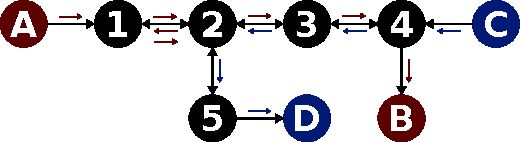
\includegraphics[width=140mm]{../img/mnv_example}
	\caption{Situace, při které neexistují cesty pro~oba agenty, aniž by se aspoň jeden vracel na navštívený vrchol}
	\label{fig:ars_mnv_example}
\end{figure}

\paragraph{Povolené zastavování (\ref{par:ars_pz})}\labeltext{PZ}{par:ars_pz}
určuje, zda-li může agent stát na~místě.
Formálněji pokud dovolím zastavování, vrchol se stane sám sobě sousedem a může se vyskytovat vícekrát na~cestě za~sebou.
Jednotlivé stání na~místě se pořád započítávají jako jednotlivé návštěvy,
tudíž maximální doma stání musí být menší než~hodnota \ref{par:ars_mnv}.

\paragraph{Maximální prodleva při~cestě (\ref{par:ars_mpc})}\labeltext{MPC}{par:ars_mpc}
omezuje počet kroků strávených agentem na~křižovatce.
Nalezená trasa pro daného agenta musí trvat nejvýše $\ref{par:ars_mpc} + p$ kroků,
kde $p$ je počet kroku optimální cesty (doba jízdy v~\hyperref[par:pruh]{pruhu}).
Hodnota $0$ znamená, že agent může jet pouze cestou stejného počtu kroků
jako je počet kroků jízdy v \hyperref[par:pruh]{pruhu}.
Tento parametr slouží jako omezení hloubky prohledávání.

\paragraph{Povolené vracení (\ref{par:ars_pv})}\labeltext{PV}{par:ars_pv}
může agentovi zakázat vracet~se na~vrchol, ze~kterého přijel.
Tento parametr dovoluje agentovi pouze \uv{jízdu dopředu}, což je přirozené od~jízdy v~autě očekávat.
Formálně pokud je tento parametr nenastaven, jsou zakázány cesty obsahující $u,v,v,\dots,v,u$,
kde $u, v \in V$ a $u \neq v$.
Posloupnost vrcholů $v$ musí být dlouhá alespoň jedna, avšak není zhora omezená.

\subsubsection{Sousední stavy}\label{subsubsec:sousedni_stavy}

Nyní blíže popíšu výběr následujícího stavu.
Přesněji popíšu funkci \ref{subsubsec:sousedni_stavy}\labeltext{\textrm{neighbour\_states}}{alg:sousedni_stavy},
která dostává na~vstup stav a vrací následující množinu platných stavů.
Množina následných stavů je ovlivněna \hyperref[subsubsec:ars_parametry]{parametry}.
Avšak většinou se jedná o~podmnožinu sousedních vrcholů aktuálního vrcholu, popřípadě ještě aktuální vrchol.
Tuto~množinu budu nazývat \emph{sousedi}\labeltext{sousedi}{str:ars_sousedi}.

Pro~získání \hyperref[str:ars_sousedi]{sousedů} začnu s~množinou všech vrcholů,
do~kterých vede hrana z~vrcholu aktuálního stavu.
Budu předpokládat, že tuto množinu je jednoduše možné získat z~grafu křižovatky.
Pokud je nastavený \hyperref[subsubsec:ars_parametry]{parametr} \ref{par:ars_pz},
přidám do~množiny \hyperref[str:ars_sousedi]{sousedů} aktuální vrchol.

Agent se nesmí srazit s~žádným jiným naplánovaným agentem při~jízdě do~sousedního vrcholu.
Kolizní přejezdy jsou detekovány způsobem popsaným v~sekci \nameref{sec:kolize}.

Pro~kontrolu \hyperref[subsubsec:ars_parametry]{parametru} \ref{par:ars_mnv}
je možné projít všechny předchozí stavy až po~počáteční
a odebrat všechny vrcholy vyskytující se alespoň \ref{par:ars_mnv} krát během tohoto průchodu.
Následující pseudokód zobrazuje přesnější postup odstraňování.

\labeltext{\textrm{control\_MNV}}{alg:ars_mnv}
% @formatter:off
\begin{code}[fontsize=\footnotesize]
// MNV předem nastavená hodnota maxima návštěv vrcholu

// vstup aktuální stav, množina sousedních vrcholů
// výstup množina sousedů navštívená nejvýše MNV - 1
control_MNV(state, neighbours)
  occurs <- empty // slovník návštěv vrcholů s implicitní hodnotou 0
  predecessor <- state
  while predecessor is not NULL
    occurs[predecessor.vertex] <- occurs[predecessor.vertex] + 1
    predecessor <- predecessor.parent
  for vertex in neighbours
    if occurs[vertex] >= MNV
      neighbours.remove(vertex)
  return neighbours
\end{code}
% @formatter:on

Pokud je hodnota \hyperref[subsubsec:ars_parametry]{parametru} \ref{par:ars_mpc} konečná,
je možné provést filtrování sousedních vrcholů podle nejkratší vzdálenosti ze~souseda do~nejbližšího cíle.
Tuto vzdálenost vím díky heuristice, která má stejnou hodnotu.
Nejprve si spočítám maximální krok cesty\labeltext{MKC}{str:ars_mkc} (\ref{str:ars_mkc}) pro~daného agenta.
Pokud sečtu aktuální plánovaný krok s~hodnotou heuristiky počátečního vrcholu, dostanu nejmenší krok,
ve~kterém se může agent dostat do~nejbližšího cíle.
\ref{str:ars_mkc} přiřadím součet této hodnoty a \ref{MPC}.
Jednoduše je vidět, že agent nemůže dorazit do~cíle po~kroku \ref{str:ars_mkc},
aniž~by porušil podmínku určenou parametrem \ref{alg:ars_mpc}.

Následně mohu zkontrolovat, jestli se agent může dostat ze~sousedního vrcholu
do~některého cíle do~kroku \ref{str:ars_mkc}.
Vzdálenost souseda do~nejbližšího cíle zjistím z~heuristiky.
Tudíž stačí porovnat součet kroku stavu a heuristiky souseda s~hodnotou \ref{str:ars_mkc}.
Přesný vzhled filtrace je popsán v následujícím pseudokódu.

\labeltext{\textrm{control\_MPC}}{alg:ars_mpc}
% @formatter:off
\begin{code}[fontsize=\footnotesize]
// MKC předem spočtená hodnota maximálního kroku cesty
// heuristics množina vzdáleností do nejbližšího cíle indexovaná vrcholy

// vstup aktuální stav, množina sousedních vrcholů
// výstup množina sousedů dostatečně blízkých cílům
control_MPC(state, neighbours):
  for vertex in neighbours
    if state.step + heuristics[vertex] >= MKC:
      neighbours.remove(vertex)
  return neighbours
\end{code}
% @formatter:on

Poslední filtrování sousedů probíhá pouze, pokud je nastaven
\hyperref[subsubsec:ars_parametry]{parametr} \ref{par:ars_pv}.
Opět lze při~kontrole využít procházení předchozích stavů.
Přesněji nejprve naleznu nejpozději navštívený vrchol před~aktuálním.
Pokud takový vrchol neexistuje, mohu skončit.
Jinak odeberu tento vrchol ze~sousedů.
Následující pseudokód zobrazuje přesnější průběh.

\labeltext{\textrm{control\_PV}}{alg:ars_pv}
% @formatter:off
\begin{code}[fontsize=\footnotesize]
// PV předem nastavená hodnota parametru povolení vrácení

// vstup aktuální stav, množina sousedních vrcholů
// výstup množina sousedů s odebraným předchozím vrcholem
control_PV(state, neighbours)
  if PV
    return neighbours
  predecessor <- state.parent
  while predecessor is not NULL and predecessor.vertex is state.vertex
    predecessor <- predecessor.parent
  if predecessor is not NULL
    neighbours.remove(predecessor.vertex)
  return neighbours
\end{code}
% @formatter:on

Nyní již můžu definovat funkci \ref{alg:sousedni_stavy} jako funkci, která vygeneruje validní sousední stavy.
Funkce nejprve pomocí funkce \textrm{neighbours} vygeneruje sousední vrcholy.
Poté~odstraní neplatné sousedy funkcemi \textrm{collision\_free},
\ref{alg:ars_mnv}, \ref{alg:ars_mpc} a \ref{alg:ars_pv}.
Nakonec pro~každý zbylý vrchol vytvoří nový stav.

Pro~vytvoření následujícího stavu je potřeba znát
úhel mezi vrcholy předchozího stavu, aktuálního stavu a dotyčného sousedního vrcholu.
Přesný výpočet zde vynechám.
Budu předpokládat, že se mohu zeptat grafu křižovatky na~tento úhel.

Pseudokód celkové funkce na~generování sousedních stavů je níže.


% @formatter:off
\begin{code}[fontsize=\footnotesize]
// G graf křižovatky
// funkce angle(u, v, w) na výpočet úhlu mezi třemi vrcholy
// heuristics množina vzdáleností do nejbližšího cíle indexovaná vrcholy

// vstup aktuální stav, poloměr agenta
// výstup množina sousedních stavů
neighbour_states(state, da)
  neighbours <- neighbours(state)
  neighbours <- collision_free(state, neighbours, da)
  neighbours <- control_MNV(state, neighbours)
  neighbours <- control_MPC(state, neighbours)
  neighbours <- control_PV(state, neighbours)

  current_vertex <- state.vertex
  last_vertex <- NULL
  if state.parent is not NULL
    last_vertex <- state.parent.vertex
  states <- empty

  for vertex in neighbours
    neighbour_state <- new
    neighbour_state.step <- state.step + 1
    if current_vertex is vertex
      neighbour_state.distance <- state.distance
    else
      neighbour_state.distance <- state.distance + 1

    angle <- 0
    if last_vertex is not NULL
      angle <- angle(last_vertex, current_vertex, vertex)
    neighbour_state.angle <- state.angle + angle
    if angle is 0
      neighbour_state.turns <- state.turns
    else
      neighbour_state.turns <- state.turns + 1
    neighbour_state.heuristics <- heuristics[vertex]
    states.add(neighbour_state)

  return states
\end{code}
% @formatter:on

\subsubsection{Výsledný algoritmus}\label{subsubsec:ars_vysledny_algoritmus}

Nakonec popíšu kompletní upravený \nameref{subsec:individualni_a_star} algoritmus.

Pro~zrychlení prohledávání použiji \emph{graph-search} variantu \nameref{sec:a_star} algoritmu.
V~této variantě si algoritmus pamatuje navštívené stavy (stavy odebrané z~fronty).
Z~množiny sousedních stavů je možné odebrat všechny navštívené stavy.
U tohoto algoritmu jsou stavy totožné, pokud mají stejný vrchol, stejný krok a zároveň vrcholy všech předků si odpovídají.
Nutnost shody všech předků vyplývá z použití dodatečných parametrů, které omezují množinu sousedů.
Například pokud se dostanu na stejný vrchol ve stejný krok ze dvou různých vrcholů
a povolím pouze jedno navštívení vrcholu, sousední stavy se u obou variant budou lišit.

Během testování jsem zjistil, že kontrola pouze rovnosti posledního vrcholu a předchozího stavu
značně zrychluje běh algoritmu, aniž by~se výrazně zhoršilo plánování.
Proto jsem se rozhodl udělat kompromis a určit, že dva stavy jsou si rovné právě tehdy,
když mají stejný vrchol, krok, a jejich rodiče mají stejný vrchol.

Nejprve je nutné pro~daného agenta spočítat heuristiku pro~každý vrchol.
To mohu provést procházením přes~cílové vrcholy.
Pro~každý cíl spočtu vzdálenost od~každého vrcholu do~tohoto cíle.
Pokud je tato hodnota menší než zatím nejmenší nalezená vzdálenost, přepíši tuto hodnotu.
Pro~účely počítání vzdálenosti mezi vrcholy si můžu tyto vzdálenosti uložit předem ke~grafu.
Tyto hodnoty lze získat například Floyd–Warshallovým algoritmem (\citet*{Floyd-Warshall}).
Poté se spočte hodnota posledního kroku \ref{str:ars_mkc} a uloží se pro~pozdější použití.

Následně algoritmus vygeneruje počáteční stav a přidá ho do~fronty prohledávaných stavů.
Poté~algoritmus odebere z~fronty nejmenší stav podle součtu ceny cesty do~vrcholu stavu a heuristiky.
Pokud vrchol odebraného stavu je mezi cílovými, zkonstruuje se cesta a přiřadí se agentovi.
Plánování agenta je v~tomto případě hotové, už~zbývá jen přidat naplánovanou cestu
do~\hyperref[par:obsazene_pozice]{tabulky obsazených pozic}, aby nedošlo ke~kolizi s~pozdějšími agenty.
Agent je následně vrácen zpět \hyperref[sec:simulace]{simulátoru}.

Pokud vrchol stavu není mezi cílovými,
získají se pomocí výše popsaného postupu sousední stavy a přidají se do~fronty.
Takto algoritmus pokračuje, dokud nenalezne validní cestu, nebo není fronta prázdná.
V~tom případě nemůže být agent naplánován, jeho cestování je pozdržené, a simulátoru se vrátí $NULL$.

Konstrukci cesty provedu postupným procházením předků koncového stavu.
Pro~každý takový stav přidám na~začátek cesty vrchol zmíněného stavu.
Tento postup budu opakovat, dokud nenarazím na předka s rodičem $NULL$.
Tento postup nazvu \ref{alg:ars_construct_path}\labeltext{\textrm{construct\_path}}{alg:ars_construct_path}.

% @formatter:off
\begin{code}[fontsize=\footnotesize]
// vstup finální stav cesty
// výstup kompletní cesta z vrcholů
construct_path(state)
  path <- empty
  while state is not NULL
    path.addFirst(state.vertex)
    state <- state.parent
\end{code}
% @formatter:on


Následující pseudokód zachycuje celý \nameref{subsec:individualni_a_star} algoritmus.

% @formatter:off
\begin{code}[fontsize=\footnotesize]
// G graf křižovatky se vzdálenostmi mezi vrcholy
// MPC parametr maximální prodlevy cesty

// vstup krok, plánovaný agent
// výstup agent nebo NULL
plan_agent(step, agent)
  MKC <- step + MPC + heuristics[entry]
  da <- agent.diameter

  // prioritní fronta porovnávající prvky podle součtu ceny cesty a heuristiky
  queue <- emptyPriorityQueue
  initial_state <- empty
  initial_state.vertex <- agent.entry
  initial_state.step <- agent.step
  initial_state.heuristics <- heuristics[entry]
  queue.push(initial_state)

  while not queue.empty()
    state <- queue.pop()
    if agent.exits.contain(state.vertex)
      agent.path <- construct_path(state)
      add_planned_agent(step, agent)  // přidání agenta do obsazených pozic
      return agent
    else
      queue.addAll(neighbour_states(state, da))

  return NULL
\end{code}
% @formatter:on


%\subsection{Hromadný A* (\ref{str:a_star_arsg})}\label{subsec:hromadny_a_star}\labeltext{A*RSG}{str:a_star_arsg}

%Rozšíření A* pro více agentů, popis vylepšení.
%Parametry, pseudokód.

Tento algoritmus plánuje agenty \ref{str:rsg} strategií, čili hledá cesty pro~všechny nové agenty najednou.
Algoritmus je založen na~\nameref{sec:a_star} algoritmu.

\subsubsection{Složený hromadný A*}\label{subsubsec:arsg_slozeny_hromadny}
Předchozí \ref{str:a_star_ars} algoritmus lze poměrně jednoduše rozšířit na~variantu pro~více agentů.
Pokud potřebuji naplánovat $n$ agentů, můžu rozšířit strukturu \ref{str:a_star_ars} stavu o~vrcholy,
na~kterých se nacházejí všichni agenti.
Tedy místo jednoho vrcholu by stav obsahoval $n$-tici vrcholů.
Stav je koncový, pokud všechny vrcholy jsou v~cílových vrcholech odpovídajících agentů.

Dále potřebuji upravit hodnotu \hyperref[par:ars_vzdalenost]{vzdálenosti} jako součet vzdáleností jednotlivých agentů.
Stejným způsobem upravím hodnoty \hyperref[par:ars_uhel_zataceni]{úhlu zatáčení},
\hyperref[par:ars_pocet_zataceni]{počtu zatáčení} a \hyperref[par:ars_heuristika]{heuristiky} jako součet
odpovídajících hodnot přes všechny agenty.

Při~vytváření následujících stavů určitého stavu je nutné zjistit \hyperref[str:ars_sousedi]{sousedy} vrcholů
jednotlivých agentů stejným způsobem jako u~\ref{str:a_star_ars} (sekce \ref{subsubsec:sousedni_stavy}).
Každý prvek kartézského součinu těchto množin \hyperref[str:ars_sousedi]{sousedů} tvoří vrcholy následujícího stavu.

Oproti \ref{str:a_star_ars} je navíc nutné kontrolovat kolize mezi jednotlivými plánovanými agenty.
Pokud je nalezená kolize mezi alespoň dvěma plánovanými agenty, je daný stav zamítnut.

Bohužel prohledávací prostor má velikost $|V|^n$, kde $n$ je počet plánovaných agentů.
Například pro~čtvercovou křižovatku s~\hyperref[par:velikost_krizovatky]{velikostí} $4$,
jedním \hyperref[par:vjezdy]{vjezdem} a jedním \hyperref[par:vyjezdy]{výjezdem} (Obrázek~\ref{fig:square_type_graph})
by~měl prohledávací prostor pro~jednoho agenta velikost $24$, pro~dva agenty $576$, pro~tři $13824$.
Proto je plánování pro~velký počet agentů je téměř nemožný z~časových i~paměťových důvodů.
Naštěstí byly vyvinuty techniky na~chytřejší plánování pomocí \nameref{sec:a_star}.



%\subsection{Vylepšený Hromadný A* (\ref{str:varsg})}\label{subsec:vylepseny_hromadny_a_star}\labeltext{VA*RSG}{str:varsg}

\citeauthor{Standley_2010} se zabýval zlepšením multiagentního \nameref{sec:a_star} algoritmu.
Nakonec ve~své práci \citet*{Standley_2010} sepsal techniky, které ve~většině případů výrazně zrychlily prohledávání.
Já se zaměřím pouze na~\nameref{subsubsec:varsg_independence_detection},
jelikož dle mého názoru přináší největší zrychlení.

\subsubsection{Independence Detection}\label{subsubsec:varsg_independence_detection}

Tato metoda rozdělí plánované agenty do~skupin.
Poté nalezne cesty pro~jednotlivé skupiny zvlášť bez~ohledu na~ostatní skupiny.
Když jsou všechny skupiny naplánovány, hledají se kolize mezi jednotlivými skupinami.
Pokud nejsou žádné kolize nalezeny, všichni agenti mají už naplánovanou validní cestu.
Jinak existuje kolize mezi agenty dvou skupin.

V~tom případě zkusí algoritmus přeplánovat první skupinu v~kolizi tak,
aby už žádný agent z~této skupiny neměl kolizní trasu s~žádným agentem první i druhé skupiny.
Pokud se nepodařilo takové trasy najít, algoritmus zkusí najít nové trasy pro~agenty druhé skupiny.
Jestliže se nepodařilo úspěšně přeplánovat ani druhou skupinu, spojí se obě skupiny do~jedné.
Potom se najdou trasy pro~tuto novou skupinu.
Při všech přeplánování se vždy kontrolují kolize s~agenty naplánovanými v~předešlých krocích.

Při~přeplánování by mohlo dojít k~zacyklení.
Například mám $3$ skupiny $g_1, g_2, g_3$, a $g_1$ je v kolizi s~$g_2$.
Povede se mi přeplánovat skupinu $g_1$,avšak nyní je $g_1$ v~kolizi s~$g_3$.
Po~opětovném přeplánování $g_1$ může oět dojít ke~kolizi s~$g_2$.
Proto je nutné udržovat si historii skupin, se kterými byla aktuálně plánovaná skupina v~kolizi.
Při~hledání nových tras se agenti vyhýbají nejen druhé skupině, ale i všem předešlým skupinám.

\paragraph{Illegal moves table}\label{par:varsg_illegal_moves_table} je datová struktura,
kterou algoritmus používá při~přeplánování k~hledání kolize s~agenty jiné skupiny.
Struktura této tabulky je shodná se strukturou \hyperref[par:obsazene_pozice]{tabulkou obsazených pozic}.
Tudíž mohu kontrolovat kolize přejezdu stejným způsobem popsaným v sekci \ref{sec:kolize}.

Před~každým přeplánováním skupiny si algoritmus uloží pro~každý krok množinu dvojic vrcholu a agenta.
Pro~každého agenta ze~skupiny z~historie nebo kolizní skupiny je do~tabulky přidána pro~každý krok, kdy agent cestuje,
dvojice zmíněného agenta a vrcholu z~jeho aktuální trasy, kde~se vyskytuje ve~zmíněný krok.

Kontrola sousedních vrcholů pro~jednoho agenta probíhá podobně jako při~kontrole u~\ref{str:a_star_ars}.
Avšak kromě kontroly kolize s~naplánovanými agenty pomocí \hyperref[par:obsazene_pozice]{tabulkou obsazených pozic}
se totožnými kontrolami zaručuje nekolizní přejezd s~agenty jiných skupin pomocí
\hyperref[par:varsg_illegal_moves_table]{Illegal moves table}.

K~rychlejšímu naplánování chceme minimalizovat počet přeplánování.
Proto by bylo vhodné již při~plánování skupiny preferovat cesty,
které mají co~nejméně kolizních tras s~ostatními skupinami.
Přesněji je důležitý počet agentů jiných skupin, které kolidují s~některým agentem aktuální skupiny.
Avšak pro~zaručení optimality je nutné dodržovat stejné uspořádání jako při~\nameref{str:a_star_arsg}.
Porovnání na~počet kolizních agentů tedy budu používat jenom tehdy, mají-li stavy totožnou
\hyperref[par:ars_vzdalenost]{vzdálenost}, \hyperref[par:ars_uhel_zataceni]{úhlu zatáčení},
\hyperref[par:ars_pocet_zataceni]{počtu zatáčení} i \hyperref[par:ars_heuristika]{heuristiku}.
Pokud bude shodný i~počet agentů s~kolizní trajektorií, budu upřednostňovat stavy s~menším počtem celkových kolizí.
Při~tomto součtu už započítávám stejného agenta vícekrát.

\paragraph{Conflict avoidance table}\label{par:varsg_conflict_avoidance_table} je tabulka, pomocí níž
algoritmus zjišťuje množství těchto kolizí.
Strukturou je podobná struktuře \nameref{par:varsg_illegal_moves_table}.
Agenti jiných skupin mohou ale být v~kolizi, proto může být naplánováno více agentů na~stejném vrcholu ve~stejný krok.
Proto je výhodnější pamatovat si místo dvojice vrchol-agent dvojici vrchol-množina agentů.
Zjišťování kolizních agentů lze opět provést podobnými způsoby popsanými v sekci \nameref{sec:kolize}.
Rozdíl je jenom namísto kontrolování s~jedním agentem
se musí zkontrolovat kolize se všemi agenty v~dané množině.

Algoritmus potřebuje na~začátku výpočtu rozdělit agenty do~skupin.
Vhodný způsob rozdělení je přiřazení každému agentovi svojí skupinu,
protože složitost plánování roste exponenciálně s~množstvím agentů ve~skupině.
Všichni agenti jsou naplánováni zvlášť stejným stejně jako u~\ref{str:a_star_ars}.
Pokud nějaký agent nemůže být naplánován, je jeho skupina vyřazena.

Může se stát, že algoritmus nebude moci najít trasy pro~všechny agenty po~spojení dvou skupin.
V~tom případě je nutné vyřadit určité agenty ze~skupiny.
Pro~zachování co nejlepších výsledků jsem se rozhodl, že budu zkoušet všechny podmnožiny agentů dané skupiny,
dokud algoritmus nenalezne trasy pro~danou podmnožinu.

\subsubsection{Parametry}\label{subsubsec:arsg_parametry}
Algoritmus má opět několik nastavitelných parametrů, kterými je možné ovlivnit chování a složitost výpočtu.
Jelikož je algoritmus rozšířením \nameref{str:a_star_ars}, ponechávám algoritmu všechny tyto parametry.
Omezení parametrem platí pro~všechny plánované agenty ve~skupině.

Počet podmnožin agentů u~spojování skupin je exponenciální.
Při~testování jsem zjistil, že algoritmu občas zabere hodně času najít vhodnou podmnožinu.
Proto jsem se rozhodl dovolit algoritmu použít zjednodušený výpočet.
Zjednodušený výpočet znamená, že algoritmus místo spojování skupin ponechá pouze skupinu větší velikosti.

\paragraph{Zjednodušený výpočet po (\ref{par:arsg_zvp})}\labeltext{ZVP}{par:arsg_zvp} je jediný nový parametr.
Tento parametr udává, po jak dlouhé prodlevě (ms) má algoritmus začít používat zjednodušené počítání.

\subsubsection{A*OID}\label{subsubsec:a_star_aoid}
Další způsob řešení \nameref{subsubsec:online_mapf} problému je pomocí \ref{str:oid} algoritmu.
Při~tomto způsobu řešení se v~novém kroku plánují nejen noví agenti, ale i agenti již naplánovaní.
Tento způsob by měl dávat lepší výsledky než \ref{str:varsg}.
Ale přirozeně vzroste počet plánovaných agentů, což vede ke~zpomalení výpočtu.
Proto \ref{str:oid} používá strategii \uv{neměnit plány agentů, pokud není potřeba}.
Znamená to, že naplánovaní agenti se znovu neplánují, jestliže nekolidují s~novými agenty.

\nameref{str:varsg} algoritmus lze jednoduše rozšířit na~\ref{str:oid} variantu.
Na~začátku každému naplánovanému agentovi přidělíme vlastní skupinu.
Avšak oproti novým agentům pro ně prvotní cestu nehledáme, jelikož už jsou naplánovaní předchozími kroky.
Akorát jejich aktuální cesta nezačíná ve~vrcholu vjezdu,
ale obecným vrcholem podle toho, kde se v~plánovaný krok nacházejí.
Množina koncových vrcholů je stejná.

Poté může algoritmus pokračovat stejně jako v~\ref{str:a_star_arsg}.
Jediný rozdíl je u~slučování dvou skupin.
Algoritmus si nemůže dovolit odebrat agenta z~výpočtu a zamítnout ho, jelikož už je částečně naplánován.
Z~tohoto důvodu se při~slučování skupin neprochází všechny podmnožiny agentů skupin,
ale jenom podmnožiny obsahující všechny dříve naplánované agenty.

Algoritmus opět podporuje \hyperref[par:arsg_zvp]{zjednudušený výpočet}.
Avšak tentokrát namísto ponechávání větší skupiny
algoritmus skupiny spojí do~jedné a odebere všechny nově plánované agenty.
Zbylí agenti již byli naplánovaní v~předešlých krocích, tudíž jim algoritmus přiřadí zpět poslední platné cesty.
Tyto cesty jsou vzájemně nekolizní, jelikož jsou výsledkem předešlých úspěšných plánování.

Abych snížil počet přeplánovaných agentů, rozhodl jsem se přidat algoritmu dva nastavitelné parametry.

\paragraph{Maximální počet agentů (\ref{par:aoid_mpa})}\labeltext{MPA}{par:aoid_mpa} určuje,
s~kolika agenty může algoritmus nanejvýš počítat.
Algoritmus přidá k~novým agentům tolik naplánovaných, abych jejich součet nepřekročil tuto hodnotu.
Výběr agentů pro~plánování tedy probíhá ještě před započtením výpočtu tras.
Agenti se berou od~nejnovějšího po~nejstarší.

\paragraph{Počet přeplánovaných kroků (\ref{par:aoid_ppk})}\labeltext{PPK}{par:aoid_ppk}
omezuje stáří přeplánovaných agentů.
Z~vybraných agentů na~přeplánování jsou odebráni takoví, kteří už cestují déle než hodnota tohoto parametru.


%\subsection{Conflict-Based Search (\ref{str:cbs})}\label{subsec:conflict_based_search}\labeltext{CBS}{str:cbs}

%Popis algoritmu, úprava pro můj problém.
%Parametry, pseudokód.

\nameref{subsec:conflict_based_search} algoritmus \citep*{Sharon} rozšiřuje jakýkoliv \ref{str:rs} algoritmus
na multiagentní plánování.
V mém případě budu rozšiřovat \ref{str:a_star_ars}.

\ref{str:cbs} začíná individuálním naplánováním všech agentů nezávisle na~sobě.
Čili agenti nesmějí mít kolize s~již cestujícími agenty,
avšak mohou mí kolizní trajektorii s~jinými aktuálně plánovanými agenty.
Poté se zkontroluje, zda-li nemají nějací agenti kolizní trajektorie.
Pokud ne, plánování úspěšně končí.
Jinak se prohledávání rozdělí na dva případy.
V obou případech je přeplánován jeden agent s podmínkou, že se musí vyhnout koliznímu místu.
Poté se opakuje opětovné hledání kolizí a rozdělování na případy.
Aby nedošlo k zacyklení, je nutné při plánování agenta vyhnout se nejen aktuální kolizi, ale také všem předchozím.
Výpočet postupně vytváří strom,
kde každý vrchol obsahuje cesty agentů (mohou být navzájem kolizní) a tabulku zakázaných pozic.
Algoritmus skončí v~prvním nalezeném vrcholu neobsahujícím kolizní trasy.

Již cestující agenti mohou omezovat trasy natolik, že pro agenta neexistuje žádná nekolizní cesta skrze křižovatku.
Dále se může stát, že agent nenajde žádnou nekolizní cestu, která by nevedla místo, které bylo dříve označené jako kolizní.
V obou případech plánování tohoto agenta selže a agent zcela odstraněn z~vrcholu.
Následně jsou nalezeni agenti, kteří byli v~historii přeplánováni kvůli odstraněnému agentovi.
Pro~tyto agenty jsou nalezeny nové cesty, jelikož pro~ně může existovat lepší cesta.

Algoritmus postupně prochází listy stromu výpočtu.
Pořadí průchodu je určeno počtem agentů.
Pokud je počet agentů u~více listů shodný, vybere se vrchol s nejmenší vzdáleností podobně jako u \ref{str:a_star_arsg}.
Algoritmus naplánuje pouze agenty, kteří mají cesty ve~vybraném listu, vjezd zbylých agentů je zamítnut.

\ref{str:cbs} najde optimální cestu pro všechny agenty \citep{Sharon}.
Avšak velikost stromu může být obrovská.
Proto jsem se rozhodl obětovat optimalitu a zjednodušit práci algoritmu, pokud plánování trvá příliš dlouhou dobu.
Ve zjednodušeném režimu algoritmus přeplánuje takovým způsobem, aby neměl žádné kolize s ostatními plánovanými agenty.
To znamená, že v tomto režimu plánuje algoritmus agenty stejně jako \ref{str:a_star_ars}.


\subsubsection{Parametry}\label{subsubsec:cbs_parametry}

\nameref{subsubsec:cbs_parametry} algoritmu jsou stejné jako u \ref{str:varsg} a mají podobný význam.
Hodnoty Maximum návštěv vrcholu (\ref{str:ars_mnv}), Povolené zastavování (\ref{str:ars_pz}),
Maximální prodleva při~cestě (\ref{str:ars_mpc}) a Povolené vracení (\ref{str:ars_pv})
algoritmus používá při~plánování jednoho agenta.
Tyto \hyperref[subsubsec:ars_parametry]{parametry} ovlivňují plánování stejně jako u \ref{str:a_star_ars}.
Hodnota parametru \ref{str:arsg_zvp} opět určuje po jak dlouhé prodlevě má algoritmus přejít na zjednodušené plánování.

\subsection{CBS-OID}\label{subsec:cbsoid}

\ref{str:cbs} lze podobně jako \ref{str:varsg} rozšířit na \ref{str:suboid} variantu.
K plánovaným agentů se přidají agenti z předchozích kroků.
Jako počáteční cesty těchto agentů se použijí jejich již naplánované trasy, tudíž se znova nepočítají.
Výpočet je poté shodný, až na~případy, kdy pro~ně nebyla nalezena cesta.
Pokud k~takové situaci dojde, namísto odstranění agenta se odstraní celý list ze~stromu výpočtu.

Parametry jsou rozšířené stejně jako u \nameref{subsubsec:a_star_aoid} o~Maximální počet agentů (\ref{str:aoid_mpa})
a Počet přeplánovaných kroků (\ref{str:aoid_ppk}).
Význam těchto parametrů je shodný.



\section{SAT planner}\label{sec:sat_planner}

%Definice SAT a MAXSAT, popis řešiče.
%Rozdíl mezi optimálním ohodnocením a splňujícím ohodnocením.
%
%Popis převodu problému na SAT.
%Popis parametrů a odhad na počet proměnných a počet klauzulí.
%
%Pseudokód.

SAT je známý a prozkoumaný problém, na který existují vysoce optimalizované řešiče.
Proto není úplně zcestné pokusit se problém křižovatky převést na SAT problém.

SAT\labeltext{SAT}{str:sat} se zabývá problémem určení,
zda-li existuje splňující ohodnocení výrokových proměnných logické formule.
Vstupní hodnotou je tedy výroková formule a výstupem ohodnocení proměnných takové,
že daná formule je splněná, popřípadě oznámení o nesplnitelnosti formule.
Zadaná formule většinou bývá v konjunktivní normální formě (\ref{str:sat_cnf})\labeltext{CNF}{str:sat_cnf}, což je konjunkce klauzulí.
Klauzule jsou disjunkce literálů a literál je výroková proměnná, nebo její negace.
Například formule v \ref{str:sat_cnf} pro proměnné $p_1, \dots, p_{10}$ může být
\[
	\bigwedge_{i=1}^{7}(p_i \vee p_{i+1} \vee p_{i + 3}).
\]

MAXSAT je rozšíření \ref{str:sat}.
Klauzule jsou rozdělené na dvě skupiny,
\ref{str:sat_hard}\labeltext{\emph{hard}}{str:sat_hard} a \ref{str:sat_soft}\labeltext{\emph{soft}}{str:sat_soft}.
Aby bylo ohodnocení splňující, musí být splněny všechny \ref{str:sat_hard} klauzule.
Úkolem řešiče je nalézt splňující ohodnocení, které maximalizuje počet splněných \ref{str:sat_soft} klauzulí.
Tento problém je očividně těžší, jelikož nestačí najít libovolné řešení, ale to nejlepší.

Vážený MAXSAT přidává navíc možnost přiřadit \ref{str:sat_soft} klauzulím váhy.
Řešič se nesnaží maximalizovat počet splněných klauzulí, ale součet jejich vah.

Pokud chceme naplánovat agenty pomocí váženého MAXSAT, stačí převést plánování do \ref{str:sat_cnf}.
Převedení \ref{str:mapf} problému na \ref{str:sat_cnf} bylo mnohokrát popsáno \citep{bartak}.
Z tohoto postupu budu vycházet.

\subsection{Převod do \ref{str:sat_cnf}}\label{subsec:sat_prevod_do_cnf}

Vhodný začátek převodu je nadefinování výrokových proměnných.
Poté popíšu tvorbu klauzulí.

\subsubsection{Výrokové proměnné}\label{subsubsec:sat_vyrokove_promenne}

Vytvořím si výrokové proměnné pro každého agenta, pro každý krok a pro každý vrchol grafu.
Pokud se agent $a$ vyskytuje v čase $t$ na vrcholu $v$, je výroková proměnná $p_{t,a,v}$ pravdivá, jinak je nepravdivá.
Avšak abych nedostal nekonečnou \ref{str:sat_cnf}, určím si maximální dobu cesty \ref{par:sat_mpk}.
Čas v~proměnné je počet kroků od~plánovaného kroku a má hodnotu ${0, \dots, mpk}$
Počet výrokových proměnných je celkem $(mpk + 1) * |A| * |V|$, kde $A$ je množina agentů a $V$ množina vrcholů.

\subsubsection{\ref{str:sat_hard} Podmínky}\label{subsubsec:sat_hard_podminky}

V této kapitole popíšu způsob, jak vytvořit odpovídající \ref{str:sat_cnf}.
Avšak nebudu popisovat jednotlivé klauzule.
Namísto toho popíšu tvorbu klauzulí jednoduššími výrazy (např.\ pro každé $p_i$, maximálně jeden z $p_i$, \ldots).
Převod těchto výrazů do validní \ref{str:sat_cnf} je triviální.
Pokud formule obsahuje některou funkci, je možné funkci vyhodnotit předem a daný výraz přidat, pokud to má smysl.

Agent přijede na vrchol \hyperref[par:vjezdy]{vjezdu} v kroku příjezdu, pokud bude úspěšně naplánován.
Zároveň musí být v jednom z časů ~cíli, aby byla cesta kompletní.
Z toho vyplývá první podmínka pro každého agenta, která značí, že daný agent není v počáteční čas na vjezdu,
nebo je v jenom jeden čas na právě jednom výjezdu.
Matematicky:
\[
	(\forall_{a \in A}) \left(\neg p_{0,a,a_e} + \sum_{t=1}^{mpk} \sum_{f \in a_f} p_{t, a, f} = 1\right),
\]
kde $a_e$ je vrchol vjezdu agenta $a$ a $a_f$ jeho výjezdy.

Agent se nemůže nacházet na více vrcholech najednou.
Jinými slovy může být pro jednoho agenta a jeden čas maximálně jedna proměnná pravdivá:
\[
	(\forall a \in A)(\forall t \in {0, \dots, mpk})\left(\sum_{v=1}^{|V|} p_{t,a,v} \leq 1\right).
\]

Pokud je agent v určitý krok na vrcholu $v$, musí být v dalším kroku na některým vrcholu z jeho sousedů $N(v)$.
Množina sousedů může obsahovat i samotný vrchol $v$,
pokud \hyperref[par:sat_povolene_zastavovani]{povolíme zastavování}.
Toto platí až na vrcholy výjezdu, které opět pro agenta $a$ označím $a_f$, a také to neplatí pro poslední krok.
Matematickým zápisem tomu odpovídá podmínka
\[
	(\forall a \in A)(\forall t \in {0, \dots, mpk - 1})
	(\forall v \in V \setminus a_f)(p_{t,a,v} \rightarrow \vee_{n \in N(v)} (p_{t+1,a,n})).
\]

Počítání lze zrychlit zakázáním neplatných kombinací času a vrcholu.
Pro tyto účely si označím $d(u, v)$ jako délku nejkratší cesty mezi vrcholy $u$ a $v$.
Pokud mezi nimi cesta neexistuje, je hodnota $\infty$.
Agent nemůže být v čase $t$ na vrcholu vzdáleném více než $t$, jelikož se tam nemá jak dostat.
Stejně tak nemůže být v čase $t$ na vrcholu, který má vzdálenost k nejbližšímu cíli větší než $mpk - t$,
protože potom neexistuje způsob, jak se dostat do cíle včas.
Odtud plynou podmínka
\begin{gather*}
(\forall a \in A)(\forall t \in {0, \dots, mpk})(\forall v \in V)
	\\
	((d(a_e, v) > t \vee (\min_{f \in a_f} d(v, f) > mpk - t)) \rightarrow \neg p_{t, a, v}).
\end{gather*}

Nadále je nutné vyhnout se cestujícím agentům.
K tomu opět využiji funkci na kontrolu kolizí.
Projdu všechny vrcholy a pro každého agenta zjistím,
na kterých vrcholech se nesmí nacházet pomocí funkce \ref{alg:kol_prejezd_mnozina}:
\[
	(\forall a \in A)(\forall t \in {0, \dots, mpk - 1})(\forall u \in V)(\forall v \in N(u))
	(\neg \ref{alg:kol_prejezd_mnozina}(a_p + t, u, v, a_d, T) \rightarrow \neg p_{t, a, u}),
\]
kde $a_p$ je krok příjezdu agenta a $a_d$ je jeho \hyperref[par:polomer_agenta]{poloměr}
a $T$ je \nameref{par:obsazene_pozice}.

Poslední nutná podmínka je zamezení kolizím mezi plánovanými agenty.
Je nutné projít všechny dvojice agentů a poté všechny kombinace vrcholů a jejich sousedů.
Pokud se vrcholy nacházejí moc blízko, nemůžou se agenti vyskytovat na patřičných vrcholech v jeden čas.
Pro zjištění vzdáleností mohu využít tabulky \ref{str:kol_vzdalenosti} a \ref{str:kol_serazene_vzdalenosti}.
Tabulka \ref{str:kol_vzdalenosti} má uložené pro každé možné dva přejezdy nejbližší vzdálenosti mezi trasami
(\ref{subsec:kontrola_prejezdu_jeden_agent}).
Tabulka \ref{str:kol_serazene_vzdalenosti} má uložené pro každé dva sousední vrcholy $u$ a $v$
seřazené dvojice vrchol, vzdálenosti podle nejmenší vzdálenosti (\ref{subsec:kontrola_prejezdu_mnozina_agentu}).
Pseudokód zachycující tvorbu této podmínky:

% @formatter:off
\begin{code}[fontsize=\footnotesize]
// tabulka seřazených vzdáleností sort_dist
// minimální povolená vzdálenost agentů d
// množina vrcholů V

// seznam agentů A
add_agents_clauses(A)
  for i in 1, ..., |A|
    for j in 1, ..., i - 1
      a <- A[i]
      b <- A[j]
      d_safe = a.polomer + b.polomer + d
      for u in V
        for v in N(u)
          for p, p_dist in sort_dist[u][v]
            if p_dist > d_safe
              break
            for q in N(p)
              if d_safe <= distance[u][v][p][q]
                for t in 0, ..., mpk - 1
                  add_hard_clause(not_near(t, a, u, v, b, p, q))
\end{code}
% @formatter:on

V kódu výše používám funkci $add\_hard\_clause(not\_near(t, a, u, v, b, p, q))$,
která přidá do SAT řešiče hard podmínku $(p_{t,b,p} \wedge \_{t+1,b,q}) \rightarrow (\neg p_{t,a,u \vee p_{t+1,a,v}})$.
Tato podmínka znamená, že pokud cestuje agent $b$ v čase $t$ z $p$ do $q$,
potom nesmí agent $a$ cestovat ve stejný čas z $u$ do $v$.

\subsubsection{\ref{str:sat_soft} Podmínky}\label{subsubsec:sat_soft_podminky}

Podobně jako u všech předešlých algoritmech budu optimalizovat \ref{str:soc} metriku.
U každému agenta tedy budu chtít co nejdřívější příjezd do cíle.
Proto vytvořím jednoprvkové klauzule pro každého agenta a pro každý vrchol s cenou určenou časem.
Klauzuli v čase $t$ ($p_{t, a, v}$) přidělím váhu $mpk - t + 1$.
Tím bude mít příjezd v $t = 1$ váhu $mpk$ a v čase $t = mpk$ váhu $1$.

Abych maximalizoval počet naplánovaných agentů, vytvořím ještě pro každého agenta $a$
klauzuli $p_{0, a, a_e}$ s vahou alespoň $(mpk + 2) * (|A| - 1)$, kde $a_e$ je vrchol vjezdu agenta $a$.

\subsection{Parametry}\label{subsec:sat_parametry}

Aby byl algoritmus porovnatelný s ostatními algoritmy, přidal jsem podobné parametry použité v předešlých algoritmech.

\paragraph{Maximální počet kroků (\ref{par:sat_mpk})}\labeltext{MPK}{par:sat_mpk}
udává maximální délku plánu pro všechny agenty.

\paragraph{Maximum návštěv vrcholu (\ref{par:ars_mnv})} má stejný význam jako
parametr \ref{par:ars_mnv} u \hyperref[subsubsec:ars_parametry]{parametrů \ref{str:a_star_ars}}.
Hodnota udává maximální počet výskytů jednoho vrcholu na cestě.
Vzorcem $(\forall a \in A)(\forall v \in V)(\sum_{t=0}^{mpk} p_{t, a, v} \leq 1)$.

\paragraph{Povolené zastavování (\ref{par:ars_pz})}\label{par:sat_povolene_zastavovani} je taktéž vzatý
z \hyperref[subsubsec:ars_parametry]{parametrů \ref{str:a_star_ars}}.
Pokud je tento parametr nastaven, agent může stát na~místě.
Znamená to přidání vrcholu do množiny sousedů daného vrcholu.

\paragraph{Maximalizace} určuje, zda-li má řešič hledat libovolné splňující ohodnocení,
nebo maximalizovat váhu klauzulí.
Vypnutí optimalizace značně zrychluje výpočet, avšak může vést k mnohem horším výsledkům.
Jelikož jsem dovolil zamítnout agentovi vjezd, je možné všechny \ref{str:sat_hard} podmínky splnit
nastavením všech proměnných na $false$.

\subsection{SAT-RSG}\label{subsec:sat_rsg}
Jak název napovídá, algoritmus plánuje všechny nové agenty v daném kroku.
Počet proměnných činí na $|A| * |V| * (mpk + 1)$.
Jelikož počet proměnných vzroste lineárně, počet všech možných ohodnocení vzroste exponenciálně.
Po nalezení splňujícího ohodnocení se algoritmus podívá na proměnnou $p_{0, a, a_e}$ pro každého plánovaného agenta $a$.
Pokud je $false$, vjezd agenta je zamítnut.
Jinak se projdou všechny ostatní proměnné, a vyberou se pravdivé.
Z těch se podle $t$ sestaví cesta do prvního cíle.
Mohlo by se stát, že některé proměnné jsou nastaveny na $true$ i po čase příjezdu do cíle.
Tyto proměnné algoritmus ignoruje.


\subsection{SAT-RA}\label{subsec:sat_ra}

Plánování může proběhnout i pro již naplánované agenty pro nalezení lepších tras strategií \ref{str:ra}.
Avšak je nutné změnit určité podmínky.
Symbol $a_e$ u dříve naplánovaných agentů nese význam vrcholu, na kterém se v plánovaném kroku nachází agent.
Zároveň agent již vjel na křižovatku.
Proto je nutné zaručit, že bude naplánován.
To lze provést odstraněním $\neg p_{0, a, a_e}$ z první \ref{str:sat_hard} podmínky.
Dostanu tedy zjednodušenou podmínku:
\[
	(\forall_{a \in A}) \left(\sum_{t=1}^{mpk} \sum_{f \in a_f} p_{t, a, f} = 1\right).
\]

Zbytek algoritmu je stejný s \nameref{subsec:sat_rsg}.

